\documentclass{article}
\usepackage[utf8]{inputenc}
\usepackage{graphicx}
\usepackage[margin=1in]{geometry}
\usepackage[dvipsnames]{xcolor}
\usepackage{url}
\usepackage{hyperref}
\usepackage[numbers]{natbib} % for numeric references
\usepackage{booktabs} % for the lines in the table
\usepackage{caption}  % for the captions next to each other
\usepackage{parskip}  % no indentation, small space between paragraphs
 
\begin{document}
 
\begin{titlepage}
    \begin{center}
        \includegraphics[width=3cm]{figures/MSP-logo.jpg}
        \vspace{1cm}
 
        {\LARGE\bfseries Fell or Found?\par}
        \vspace{0.4cm}
        {\Large\bfseries A data analysis of meteorite landings\par}
 
        \vspace{1.5cm}
 
        \textbf{\Large Cassandra Bargagni (ID6442941)}
 
        \vfill
 
        \large Date: \today
 
    \end{center}
\end{titlepage}
 
\newpage
 
\section*{Introduction}
A meteorite is a fragment of rock or metal from space that survives its passage through the atmosphere and falls to Earth. Meteorites are recorded in two ways: a \textbf{Fell} meteorite was \emph{seen} falling and then collected, while a \textbf{Found} meteorite was discovered later, without anyone seeing it fall.
 
In this project, we ask: \textbf{How do meteorites observed while falling differ from those found after landing?} We compare the two groups based on how many there are, where they were recorded, and how much they weigh. We expect the differences to also depend on \emph{observational and search bias}: a meteorite catalogue records not only what falls, but also how and where people search for meteorites.
 
\section*{Data sample}
We use NASA's public dataset \emph{Meteorite Landings}~\cite{nasa}, based on the Meteoritical Bulletin Database~\cite{metbull}. It contains 45\,716 meteorites; the columns used are \texttt{fall} (Fell or Found), \texttt{mass (g)}, \texttt{reclat} (latitude) and \texttt{reclong} (longitude). The dataset is very unbalanced: 44\,609 meteorites are Found and only 1\,107 are Fell (Table~\ref{tab:results}). For this reason, we compare the groups using \textbf{percentages calculated within each group}, not raw counts.
 
The analysis is written in Python with \texttt{pandas}, \texttt{numpy} and \texttt{matplotlib}:
\begin{itemize}
  \setlength\itemsep{0pt}\setlength\parsep{0pt}
  \item \textbf{Cleaning.} For the mass analysis we only use rows with a positive mass. For the location analysis we remove missing coordinates, coordinates outside the valid range, and the point $(0,0)$, which the dataset uses for an unknown location.
  \item \textbf{Continents.} Each latitude/longitude pair is converted to a continent with the \texttt{offlineRevGeocoder} package. The coordinates are rounded to 3 decimals and saved in a dictionary, so each location is looked up only once.
  \item \textbf{Mass.} We calculate the \textbf{median} mass of each group (the middle value, which, unlike the mean, is not affected by a few very large meteorites) and the percentage of each group in five mass ranges.
  \item \textbf{Uncertainty.} For a percentage $p$ calculated from $N$ meteorites, we use the binomial uncertainty $\sigma_p = \sqrt{p(1-p)/N}$, shown as error bars in the plots.
\end{itemize}
 
\section*{Results and discussion}
\textbf{Location.} Figure~\ref{fig:continents} shows that 71.1\% of the Found meteorites with usable coordinates come from Antarctica, while \textbf{none} of the Fell meteorites do. Fell meteorites come mainly from Europe ($34.3 \pm 1.5$\%), Asia ($29.5 \pm 1.4$\%) and North America ($16.9 \pm 1.1$\%), where Found meteorites are rare.
 
\begin{figure}[ht]
  \centering
  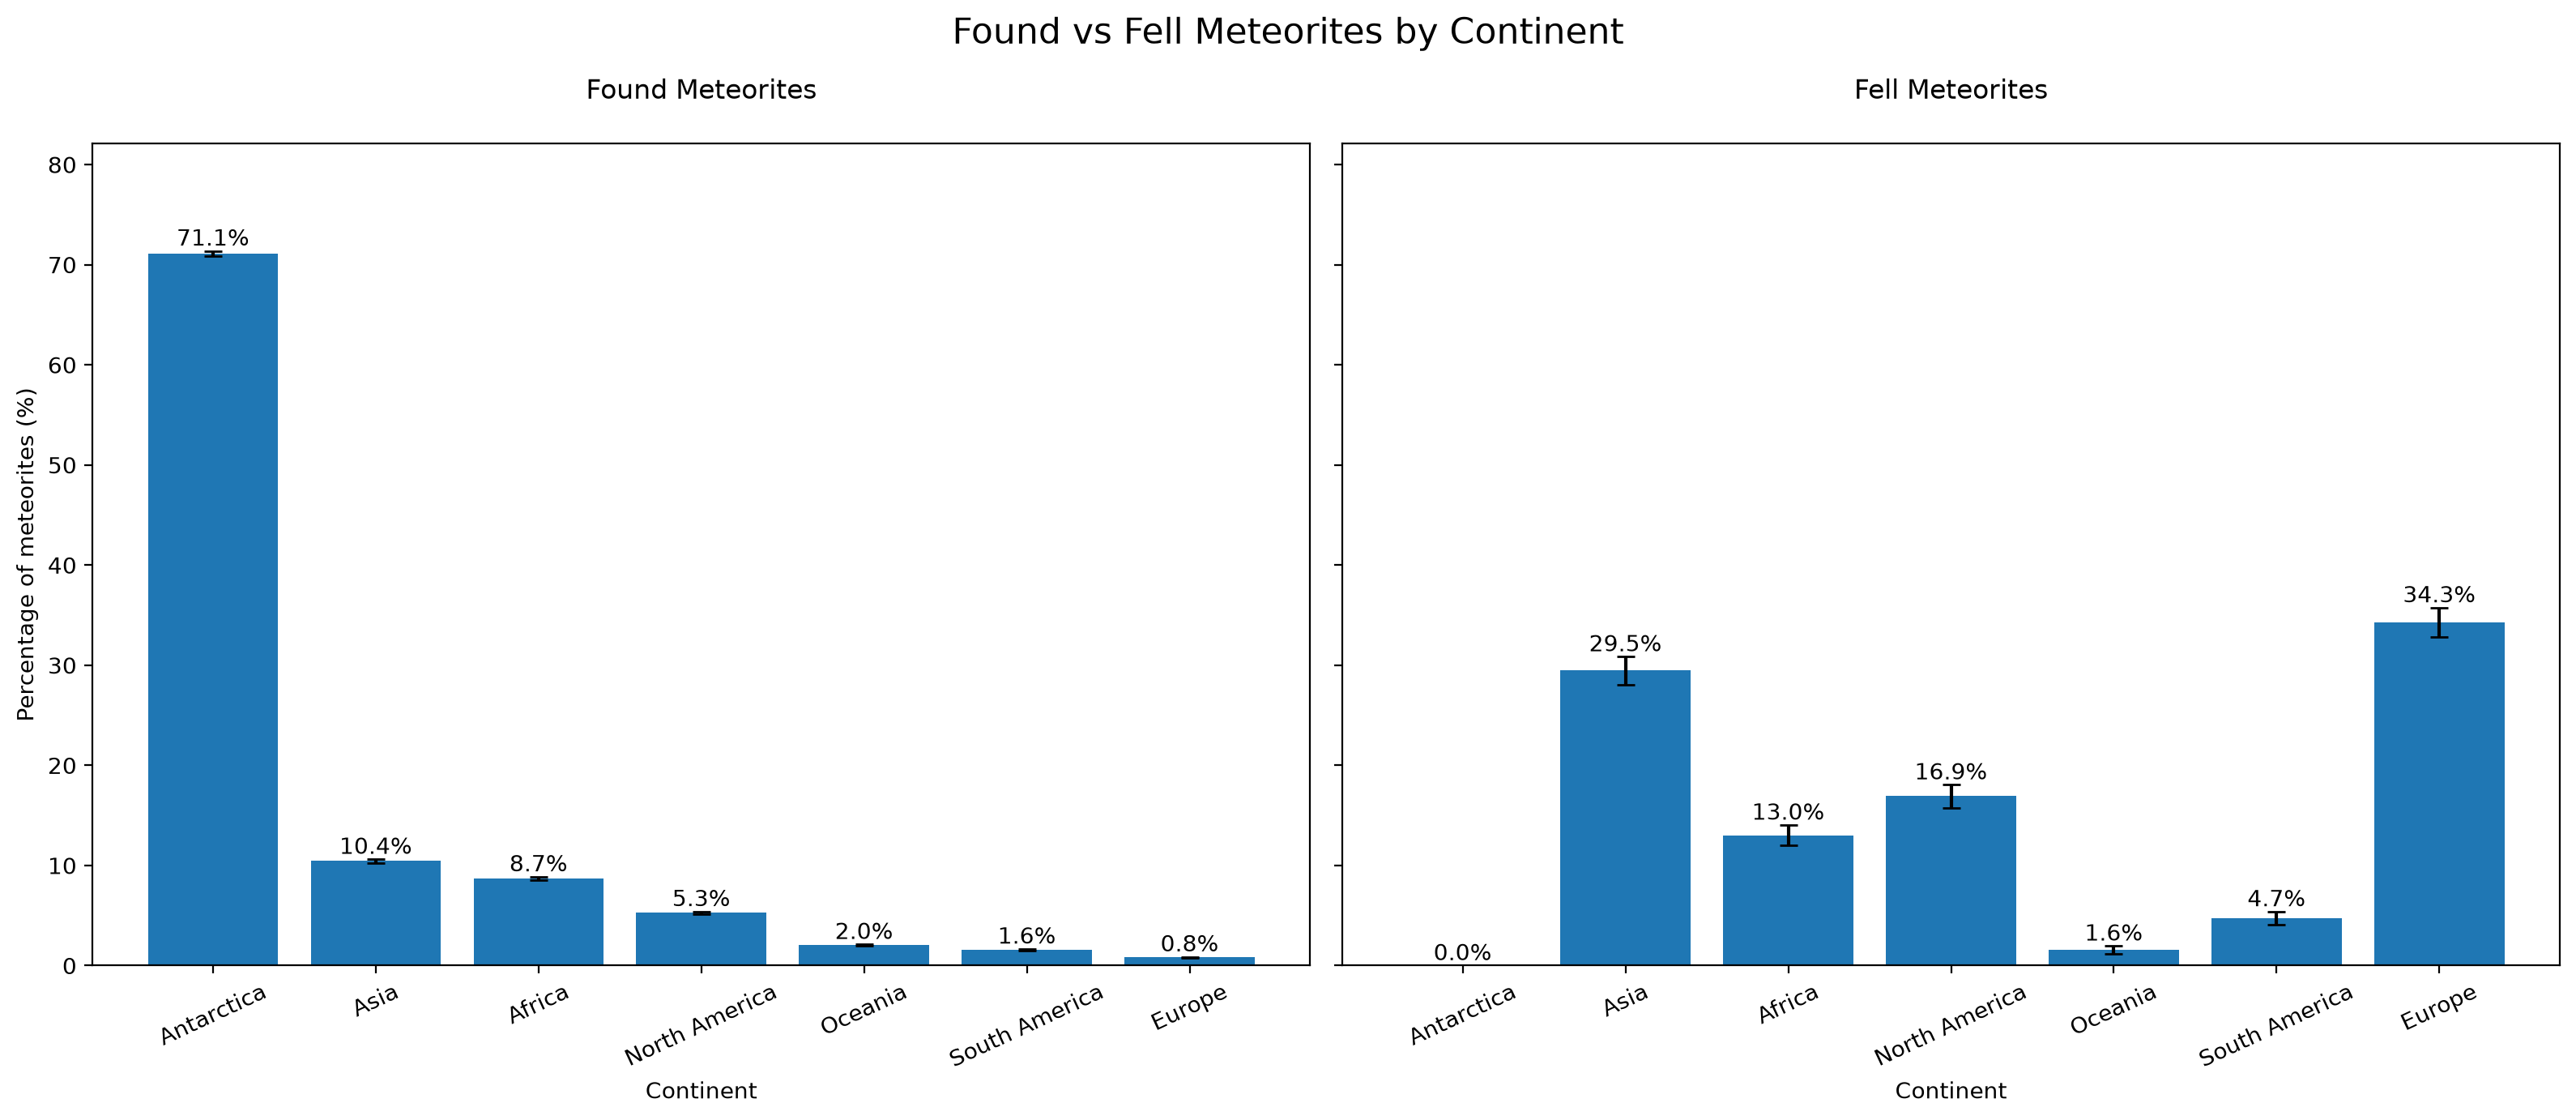
\includegraphics[width=0.95\textwidth]{plot_continents.png}
  \caption{Percentage of Found (left) and Fell (right) meteorites per continent, calculated within each group. The error bars show the binomial uncertainty $\sigma_p$.}
  \label{fig:continents}
\end{figure}
 
\textbf{Mass.} The median mass of Fell meteorites is \textbf{2\,800\,g}, compared to \textbf{30.5\,g} for Found meteorites: about 90 times larger. Figure~\ref{fig:mass} shows that this is not caused by a few extreme values: the whole distribution is different. Found meteorites are concentrated below 100\,g, while Fell meteorites are shifted towards the kilogram range.
 
\textbf{Uncertainty.} The error bars of the Fell group are larger because this group is about 40 times smaller. However, the differences between the two groups (tens of percentage points) are much larger than the error bars, so they are not due to chance (Table~\ref{tab:results}).
 
\begin{figure}[ht]
  \centering
  \begin{minipage}[c]{0.52\textwidth}
    \centering
    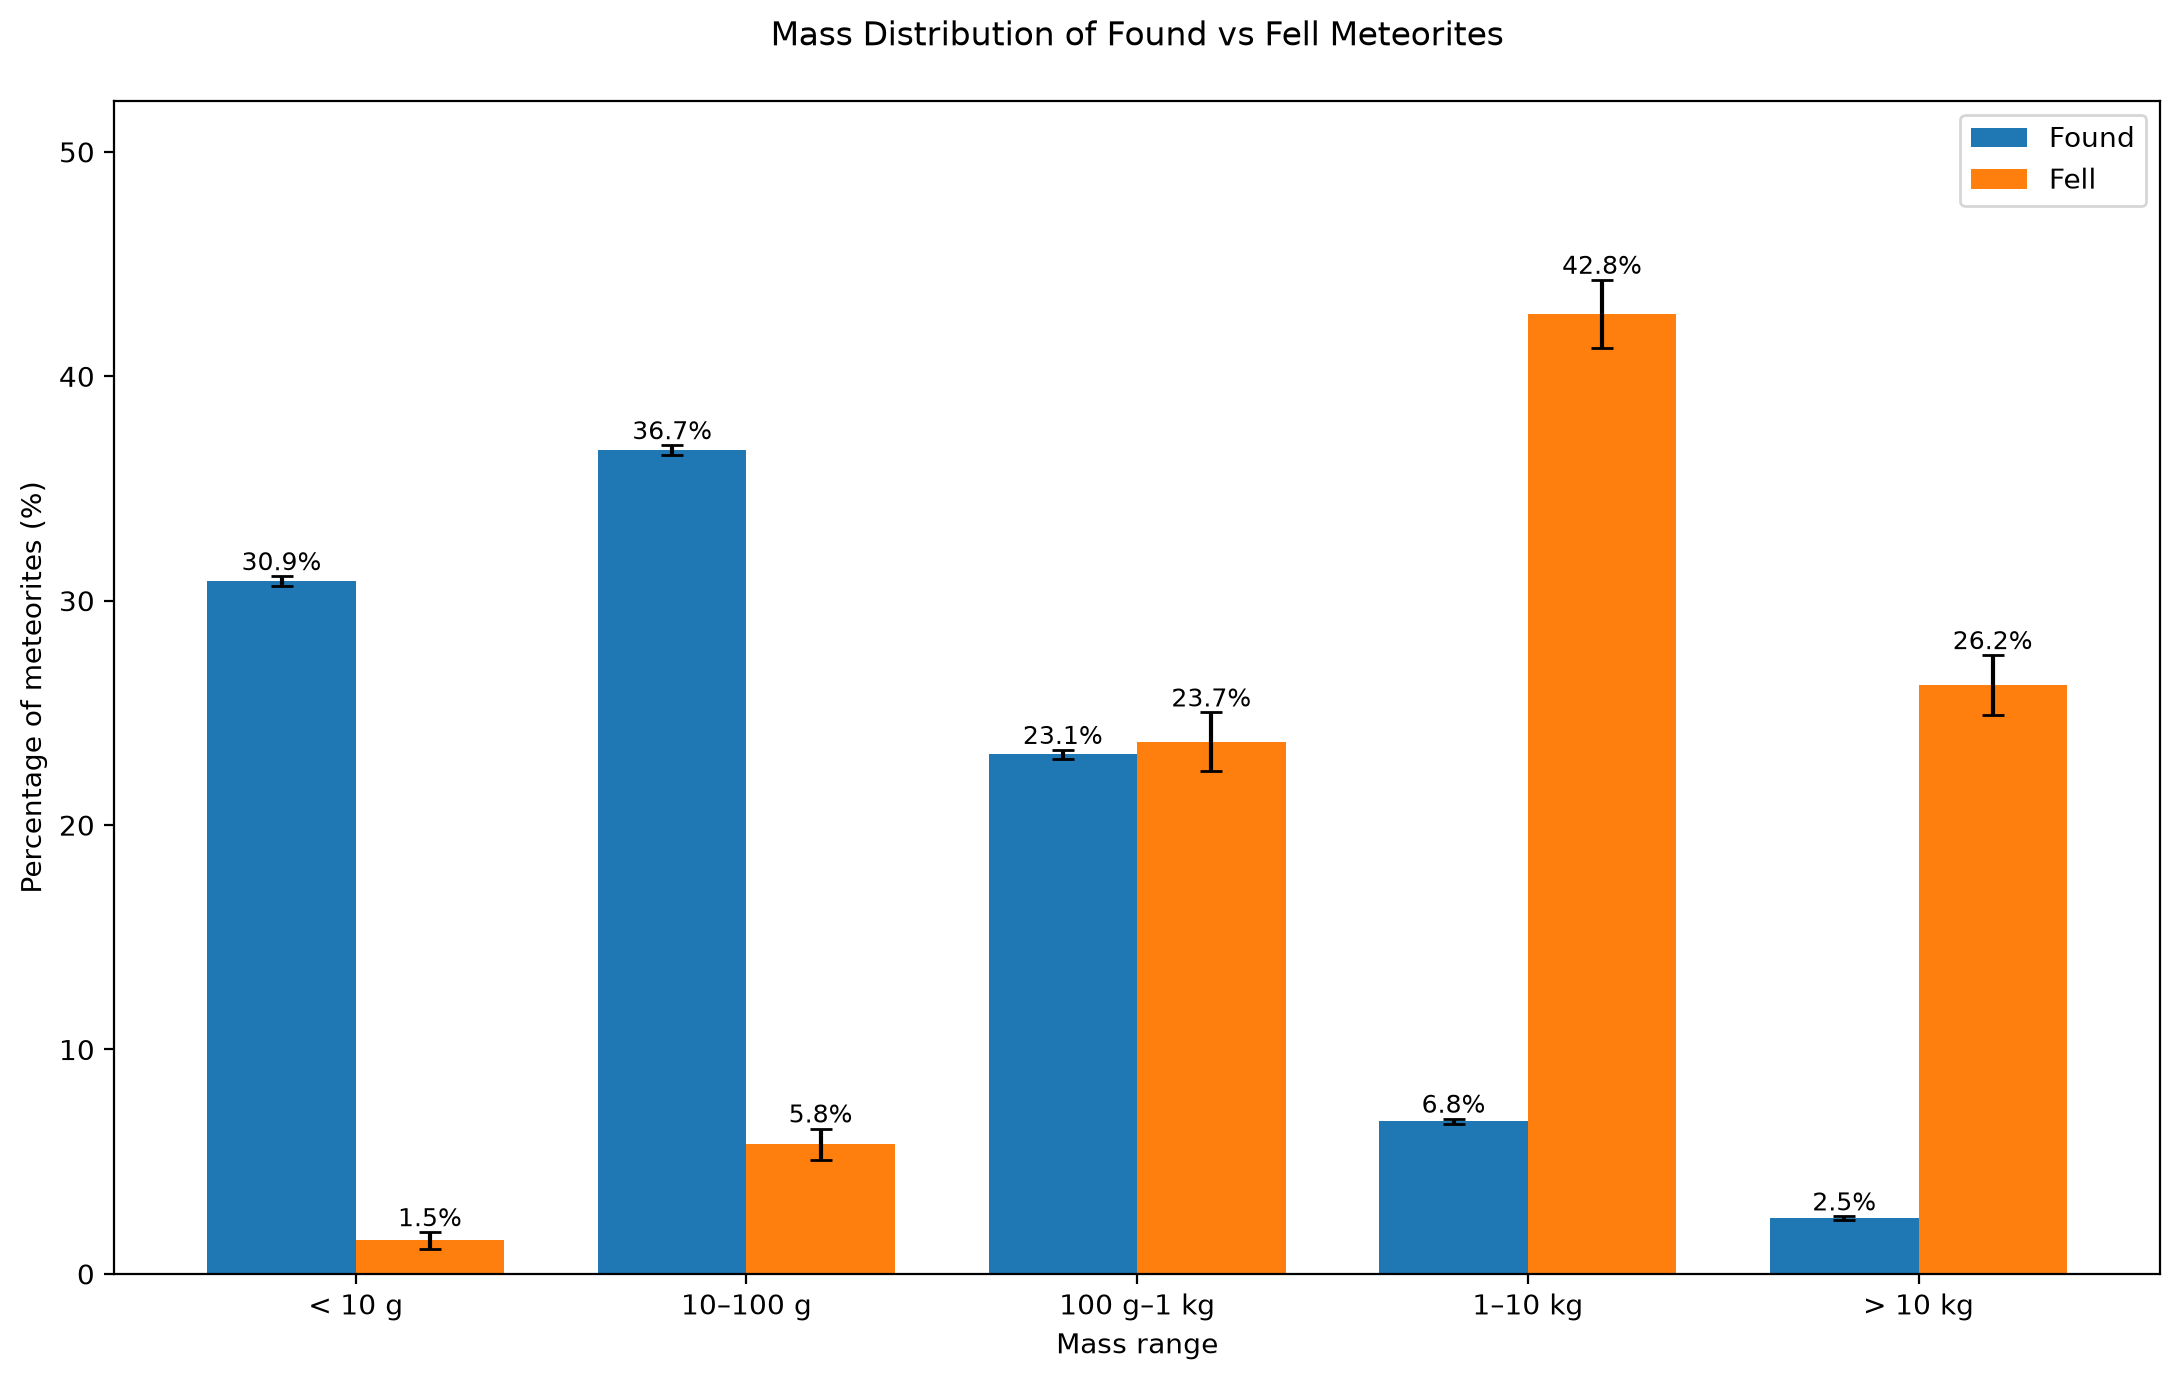
\includegraphics[width=\linewidth]{plot_mass_ranges.png}
    \captionof{figure}{Percentage of Found and Fell meteorites per mass range, with uncertainty $\sigma_p$.}
    \label{fig:mass}
  \end{minipage}
  \hfill
  \begin{minipage}[c]{0.45\textwidth}
    \centering
    \footnotesize
    \captionof{table}{Main results ($\pm\,\sigma_p$).}
    \label{tab:results}
    \begin{tabular}{lcc}
      \toprule
      & \textbf{Found} & \textbf{Fell} \\
      \midrule
      Number            & 44\,609 & 1\,107 \\
      Share of dataset  & $97.6 \pm 0.1$\% & $2.4 \pm 0.1$\% \\
      In Antarctica     & $71.1 \pm 0.3$\% & 0\% \\
      In Europe         & $0.83 \pm 0.05$\% & $34.3 \pm 1.5$\% \\
      Median mass       & 30.5\,g & 2\,800\,g \\
      Mass $<10$\,g     & $30.9 \pm 0.2$\% & $1.5 \pm 0.4$\% \\
      Mass 1--10\,kg    & $6.8 \pm 0.1$\% & $42.8 \pm 1.5$\% \\
      \bottomrule
    \end{tabular}
  \end{minipage}
\end{figure}
 
\textbf{Interpretation.} These differences \textbf{do not} mean that meteorites fall differently in different places, nor that Fell meteorites are naturally heavier. The most likely explanation is \textbf{observational and search bias}. A fall is only recorded if someone sees it, so Fell meteorites come from populated areas such as Europe and Asia. Large objects produce brighter fireballs and are easier to recover, so Fell meteorites tend to be heavier. In Antarctica, on the other hand, dark meteorites are easy to spot on the white ice, the cold preserves them, and the moving ice concentrates them in certain areas, so search expeditions recover many small meteorites. Found meteorites may also have lost mass through weathering.
 
\textbf{Limitations.} Many rows were excluded because of missing or placeholder coordinates, and the recorded mass may be the total recovered mass rather than the original mass. The error bars only describe the statistical uncertainty, not the observational bias, which is a systematic error. Furthermore, for $p=0$ (Fell meteorites in Antarctica) the formula gives zero uncertainty, which should be interpreted with caution.
 
\textbf{Conclusion.} In this dataset, Found and Fell meteorites differ strongly both in where they are recorded and in how much they weigh, and these differences are much larger than the statistical uncertainty. This pattern is probably mainly caused by how people observe and search for meteorites: the dataset tells us as much about human observation as it does about the meteorites themselves.
 
\begin{thebibliography}{9}
\bibitem{nasa}
NASA Open Data Portal. \emph{Meteorite Landings}. Available at: \url{https://data.nasa.gov/Space-Science/Meteorite-Landings/gh4g-yrr2}.
 
\bibitem{metbull}
The Meteoritical Society. \emph{Meteoritical Bulletin Database}. Available at: \url{https://www.lpi.usra.edu/meteor/}.
\end{thebibliography}
 
\end{document}